\documentclass{article}
\usepackage{graphicx}

% Required for inserting images
\usepackage{romannum}
\usepackage{hyperref}
\usepackage{multicol}
\usepackage{}
\usepackage[T2A]{fontenc}
\usepackage[english]{babel}
\usepackage{ragged2e}
\usepackage{blindtext}
\usepackage{subcaption}
\usepackage[export]{adjustbox}
\usepackage[paperwidth=230mm,paperheight=280mm]{geometry}
\usepackage{csquotes}
\usepackage[<options>]{natbib}
\addto\captionsrussian{\def\refname{}}

\geometry{
 total={180mm,200mm},
 left=25mm,
 right=25mm,
 top=21mm,
 bottom=25mm,
 }

\begin{document}
\graphicspath\ % Required for inserting images
\AtBeginDocument{\pagenumbering{arabic}}


\begin{multicols}{2}
\setlength{\hsize}{0.90\hsize}% emphasize effects
\ such semantic networks are called sc-elements (sc-nodes
and sc-connectors, which, in turn, depending on their
orientation, can be sc-arcs or sc-edges). The universality
and unification of the SC code makes it possible to
describe on its basis any type of knowledge and any
methods for solving problems, which, in turn, greatly
simplifies their integration both within one system and
within a group of such systems.
 \vspace{

} The basis of the knowledge base developed using the
OSTIS Technology is a hierarchical system of semantic
models of subject areas and ontologies, among which
stands out the universal Core of semantic models of
knowledge bases and the methodology for developing
semantic models of knowledge bases, ensuring semantic
compatibility of the developed knowledge bases [10]. The
basis of the OSTIS -system problem solver is a set of
agents that interact exclusively through the specification
of the information processes they perform in semantic
memory (sc-agents). All of these principles together
make it possible to ensure semantic compatibility and
simplify the integration of both various components of
computer systems and such systems themselves. Within
the framework of the OSTIS Technology, several universal options for visualizing SC code structures are
proposed. Within the framework of this work, examples
will be used in SCg-code - a graphical version of
visualization of SC-code constructions and SCn-code —
a structured hypertext version of visualization of SC-code
constructions.

\begin{center}
\vspace{0.2cm}

\Romannum{4}. Practical implementation of IIRS based on OSTIS
Technology (using the example of a unit for
post-treatment of wastewater from dairies — biological
ponds)
\end{center}
\vspace{0.2cm}


    

In biological ponds for post-treatment, contaminants
are removed by aerobic microorganisms, which enter
them with purified liquid from secondary settling tanks
(after aeration tanks and/or biological filters), and also
develop directly in the ponds themselves. Higher aquatic
vegetation (algae) plays an important role. The rate
of the biochemical process of extraction and oxidation
of organic pollutants in ponds with natural aeration is
limited by the low rates of atmospheric reaeration and
mass transfer processes. In ponds with artificial aeration,
as a result of supplying the required amount of air
with intensive mixing of the liquid, the speed of the
biochemical process is 5–7 times greater.
\vspace{

}The feasibility of their use at dairy processing enterprises is largely due to the fact that many harmful organic
substances are not completely oxidized at biological
wastewater treatment facilities; they remain stable in
water for a long time and can have a toxic effect on
living organisms. In addition, intensive technologies have
significant disadvantages: high energy costs for aeration
and problems associated with the processing and disposal
of large amounts of excess sludge formed, its swelling
and foaming.
\vspace{

}The characteristics of the life cycles of biological
ponds fully include: nonlinearity, nonstationarity, multifactoriality, multiprocessivity, constant changes in the
structure of internal relationships, the presence of significant hidden mutual influences between technological
parameters. Accordingly, it is justified to apply OSTIS
Technology to the creation of a knowledge base of
their processes with further synthesis of an intelligent
information and reference system.
\vspace{

}The formation of the IIRS knowledge base was based
on the national regulatory document - BS 4.04.02-2019
“Building standards of the Republic of Belarus Sewerage. External networks and structures.” Let’s consider a
fragment of the ontology that describes the concept of
“biological pond” and the parameters specified on it in
the SCn code [10]. 

\vspace{0.2cm}



\textit{\textbf{biological pond}}
\vspace{

}
$\Rightarrow$ \textit{explanation*:}
\vspace{

}
[Used for purification and post-treatment of municipal, domestic, industrial and surface wastewater
containing organic substances.]
\vspace{

}
$\Rightarrow$ \textit{subdividing*:}
\vspace{

}
\textit{$\{$• biopond with artificial aeration}
\vspace{

}
\textit{• biopond with natural aeration}
\vspace{

}
$\}$
\vspace{

}
$\Rightarrow$ \textit{parameters*:}
\vspace{

}
\textit{$\{$• waste water flow}
\vspace{

}
$\in$ \textit{measurable parameter}
\vspace{

}
$\Rightarrow$\textit{ designation*:}
\vspace{

}
[Qw]
\vspace{

}
$\Rightarrow$\textit{ measurement unit*:}
\vspace{

}
\textit{1 m3/day}
\vspace{

}
$\}$
\vspace{

}
\textbf{\textit{waste water}}
\vspace{

}
\textit{:= explanation*:}
\vspace{

}
[surface, domestic and industrial waters discharged
into sewers]
\vspace{

}
$\Rightarrow$ parameters*:
\vspace{

}
\textit{$\{$• TBOD}
\vspace{

}
$\in$ \textit{biochemical indicator}
\vspace{

}
\textit{• average monthly temperature in winter}
\vspace{

}
\textit{• average monthly temperature in summer}
\vspace{

}
$\}$
\vspace{

}
\textbf{\textit{TBOD}}
\vspace{

}
\textit{:= [total biological oxygen demand]}
\vspace{

}
$\Rightarrow$\textit{ explanation*:}
\vspace{

}
[reflects the amount of oxygen required for the biochemical oxidation of organic wastewater 
contaminants in 20 days]
\vspace{

}
$\in$\textit{ measurable parameter}
\vspace{

}
$\Rightarrow$ \textit{designation*:}
\vspace{

}
[L]
\vspace{

}
$\Rightarrow$ \textit{measurement unit*:}
\vspace{

}
$1 mg/l$

Consider for an example of using the developed ontology to describe a specific technological task. A biological
pond with a flow rate of $Qw$ = 5640 $m^3/day$ was taken as
a technological prototype. Biochemical indicators of the
processed WW: biological oxygen demand (TBOD) Len
= 18 mg/l; The technological task is to provide a TBOD
of treated wastewater Lex = 5 mg/l. At the same time,
the average monthly temperature of PW for the summer
period is Tw = 22 °C; average monthly temperature for
the winter period Tw = 15 °C. The indicated parameters
correspond to the use of a biological pond after a
fairly well-functioning biological and physico-chemical
wastewater treatment of a large milk processing plant.
Figures \Romannum{4}–\Romannum{4} show an example of a problem condition and related parameters, formalized in the SCgcode [10].

% \begin{figure}
 
 
\includegraphics[width=7.5cm]{1212122.png}
\begin{center}
    

\quote{Figure 4. Formulation of the problem conditions (fragment 2)}
  \end{center}
   
    \label{fig:enter-label}
% \end{figure}

   \begin{center}

\Romannum{5}. Conclusion
       
   \end{center}
 The use of OSTIS Technology and the development of
the corresponding ISRS in the analysis and formation of
new production knowledge in the water use segment of
dairy processing enterprises will allow:
\begin{itemize}
\item increase the efficiency and versatility of decisionmaking, including cases of complex production situations;
\item improve administration flexibility, even when expanding technological lines;
\item increase the level of qualifications of employees,
since the OSTIS Technology represents a knowledge
system in natural language and corresponds to modern ideas about the organization of human long-term
memory.\vspace{

}
\end{itemize}
Taken together, the creation of such products based
on the OSTIS Technology will form an ontological basis
for digital modeling of resource use processes (water,
electricity, heat, steam, reagents) in dairies.

\vspace{0.2cm}
\begin{center}
    

Acknowledgment
\end{center}
\vspace{0.2cm}

The authors would like to thank the scientific team
of the department of intelligent information technologies
of the Belarusian State University of Informatics and
Radioelectronics for their assistance in the work and
valuable comments.

\vspace{0.2cm}
\vspace{

}
\begin{thebibliography}{10}
\bibliographystyle{plain}
\renewcommand{\bibname}{}
\setlength{\parskip}{-0.1cm}
\linespread{0cm}
\begin{description}
\item \href{http://www.overleaf.xn--com}{ [1] Mittal S., Khan M. A., Romero D., Wuest T. Smart manufacturing: Characteristics, technologies and enabling factors. Proc.
of the Institution of Mechanical Engineers, Part B: Journal of
Engineering Manufacture, 2019, Vol. 233(5), pp. 1342–1361.
DOI:10.1177/0954405417736547.}

\item \href{http://www.overleaf.xn--com}{
[2] Grieves M., Vickers J. Digital Twin: Mitigating Unpredictable,
Undesirable Emergent Behavior in Complex Systems. Kahlen
F. J., Flumerfelt S., Alves A. (Eds). Transdisciplinary Perspectives on Complex Systems. Cham: Springer, 2017, pp. 85-113.
$DOI:10.1007/978-3-319-38756- 7_4.$}
\item \href{http://www.overleaf.xn--com}{
[3] Tao F., Zhang H., Liu A., Nee A. Y. Digital twin in industry: Stateof-the-art. IEEE Trans. on Industrial Informatics, 2019, Vol. 15,
pp. 2405-2415.}
\item \href{http://www.overleaf.xn--com}{
[4] Shtepa, V. N. Funkcional’no-staticheskij analiz sistemy kontrolja vodootvedenija i ocenka podhodov k ejo cifrovomu modelirovaniju [Functional-static analysis of the water disposal control system and assessment of approaches to its digital modeling]. Computer science and cybernetics: scientific journal, 2023,
No. 3(33), pp. 35-42.}
\item \href{http://www.overleaf.xn--com}{
[5] Shtepa V. N., Zolotykh N. Yu., Kireev S. Yu. Obosnovanie i
shemy ispol’zovanija ranzhirujushhih izmeritel’nyh sistem jekologicheskogo monitoringa i intellektual’nogo analiza rezhimov
vodootvedenija [Justification and schemes for using ranking measurement systems of environmental monitoring and intelligent
analysis of water disposal regimes]. Bulletin of Polotsk State
University. Series F. Construction. Applied sciences: scientific
journal, 2023, No. 1, pp. 94–103.}
\item \href{http://www.overleaf.xn--com}{
[6] Alekseevsky D. Enhancing Ecological Efficiency in Biological
Wastewater Treatment: A Case Study on Quality Control Information System. Water, 2023, Vol. 15, Iss. 21, P. 3744.}
\item \href{http://www.overleaf.xn--com}{
[7] Shifrin S. M., Ivanov G. V., Mishukov B. G., Feofanov Yu. A.
Ochistka stochnyh vod predprijatij mjasnoj i molochnoj promyshlennosti [Wastewater treatment of meat and dairy industry enterprises]. Light and food industry, 1981, P. 272} 
\item \href{http://www.overleaf.xn--com}{
[8] Garzanov A. L., Usov A. V., Kushniruk M. Yu., Barabash V. P.,
Kamalyan O. A. Modernizacija ochistnyh sooruzhenij fabriki
morozhenogo [Modernization of treatment facilities at an ice
cream factory]. "Morozhenoe i zamorozhennye produkty" ["Ice
cream and frozen foods"], 2004, No. 6, pp. 26-27.}
\item \href{http://www.overleaf.xn--com}{
[9] Voitov I.V. O zadachah cifrovizacii sistem vodootvedenija
kommunal’no-promyshlennyh ob’ektov [On the tasks of digitalization of water disposal systems of municipal and industrial
facilities]. Petroleum and gas chemistry – 2023: materials of
the VI International Scientific and Technical Forum on Chemical
Technologies and Oil and Gas Processing, Minsk, November 1-3,
2023, BSTU, 2023, pp. 147-151.}
\item \href{http://www.overleaf.xn--com}{
[10] V. Golenkov, Ed., Tehnologija kompleksnoj podderzhki
zhiznennogo cikla semanticheski sovmestimyh intellektual’nyhkomp’juternyh sistem novogo pokolenija [Technology of
complex life cycle support of semantically compatible intelligent
computersystems of new generation]. Bestprint, 2023.}
\end{description}
\end{thebibliography}
\end{multicols}
\begin{center}
    

    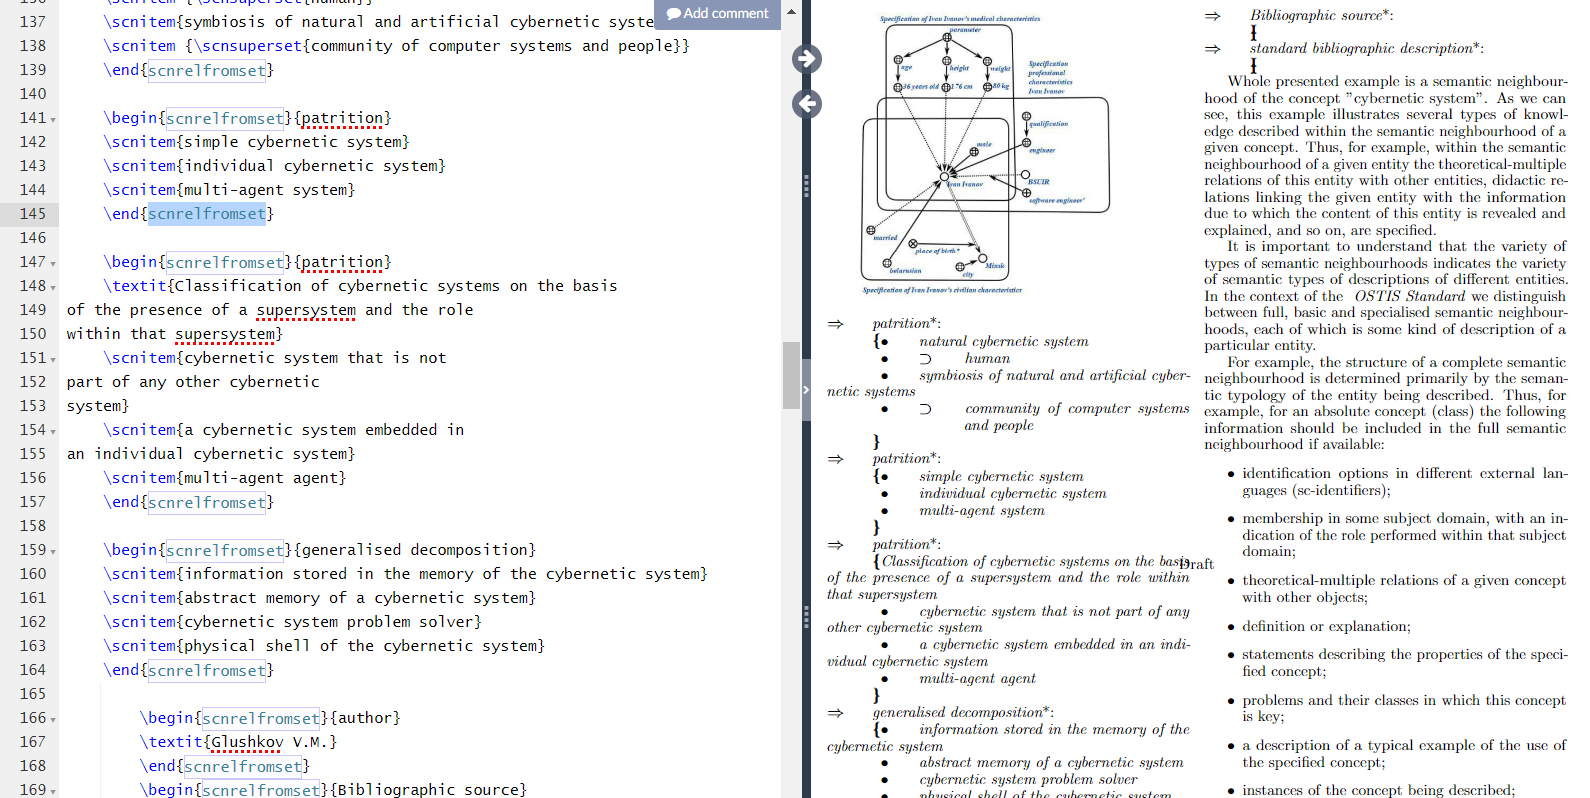
\includegraphics[width=0.6\linewidth]{image.png}

\quote{Figure 3. Formulation of the problem conditions (fragment 1)}
    \end{center}
\begin{multicols}
\maketitle{ПРИКЛАДНЫЕ АСПЕКТЫ
 ИСПОЛЬЗОВАНИЯ ТЕХНОЛОГИИ
 OSTIS ПРИ ИНФОРМАЦИОННОМ
 ОБЕСПЕЧЕНИИ ЦИФРОВИЗАЦИИ
 ПРОЦЕССОВ ВОДОПОЛЬЗОВАНИЯ
 МОЛОКОПЕРЕРАБАТЫВАЮЩИХ
 ПРЕДПРИЯТИЙ}


\vspace{0.2cm}

\begin{r}

    

\ Штепа В. Н., Муслимов Э. Н.
Оценены концептуальные подходы цифровизации производств на основе идеологии e-Manufacturing, которые предложено использовать для моделирования процессов водопользования предприятий по переработке молока, проанализированы организационно-технологические процессы формирования загрязнителей их сточных вод. В методологии IDEF0
выполнено функциональное моделирование водопользования таких производств, что позволило выявить сложность
и многонаправленность взаимосвязей параметров и обосновать использование технологии OSTIS для задач формирования интеллектуальной информационно-справочной системы.
На примере биологического пруда, как узла очистки сточных
вод, реализован элемент предложенного подхода.
\end{multicols}
\vspace{

}
Received 13.03.2024

\end{r}



\end{document}
